\documentclass[10pt]{beamer}

\usetheme{CambridgeUS}
\usepackage[english, russian]{babel}
\usepackage[utf8]{inputenc}
\usepackage{caption}
\usepackage{etoolbox}
\usepackage{multicol}
\AtBeginEnvironment{minted}{\singlespacing%
    \fontsize{10}{10}\selectfont}

\title[\href{https://goo.gl/NRgp8K}{https://goo.gl/NRgp8K} (Term 3)]{Алгоритм Касаи}
\author[Гусев Илья]{Гусев Илья}
\institute[МФТИ] 
{Московский физико-технический институт\\*}
\date{Москва, 2018}
\subject{Computer Science}

\begin{document}

\begin{frame}
  \titlepage
\end{frame}

\begin{frame}{Содержание}
\tableofcontents
\end{frame}

\section{Алгоритм Касаи}

\subsection{Задача}
\begin{frame}[fragile]{Задача}
Вычислить длину наибольших общих префиксов (LCP) для всех соседних суффиксов строки, отсортированных в лексикографическом порядке
\end{frame}

\subsection{Алгоритм Касаи}
\begin{frame}[fragile]{Алгоритм Касаи, Аримуры, Арикавы, Ли, Парка}
\begin{tabular}{ |c|c|c|c|c|c|c|c|c| } 
 \hline
 \textb{Str} & a & a & b & a & a & c & a & \# \\ 
 \hline
 \textb{Idx} & 0 & 1 & 2 & 3 & 4 & 5 & 6 & 7 \\
 \hline
  \hline
 \textb{Suf} & 7 & \color{red}{6} & \color{blue}{0} & \color{blue}{3} & 1 & \color{red}{4} & 2 & 5 \\ 
  \hline
 0 & \#& a & a & a & a & a & b & c \\ 
 1 &   & \#& a & a & b & c & a & a \\ 
 2 &   &   & b & c & a & a & a & \#\\ 
 3 &   &   & a & a & a & \#& c &   \\ 
 4 &   &   & a & \#& c &   & a &   \\
 5 &   &   & c &   & a &   & \#&   \\
 6 &   &   & a &   & \#&   &   &   \\
 7 &   &   & \#&   &   &   &   &   \\
 \hline
  \hline
 \textb{LCP} & \# & 0 & 1 & 2 & 1 & 1 & 0 & 0 \\ 
 \hline
\end{tabular}\\
\vspace{5mm}
Утверждение 1: $\forall x<y \leq z, LCP(S_{Suf[y-1]},S_{Suf[y]})\geq LCP(S_{Suf[x]},S_{Suf[z]}) $\\
Пример: LCP(S_3, S_0) \geq LCP(S_4, S_6)
\end{frame}

\begin{frame}[fragile]{Алгоритм Касаи, Аримуры, Арикавы, Ли, Парка}
\begin{tabular}{ |c|c|c|c|c|c|c|c|c| } 
 \hline
 \textb{Str} & a & a & b & a & a & c & a & \# \\ 
 \hline
 \textb{Idx} & 0 & 1 & 2 & \color{magenta}{3} & 4 & 5 & 6 & 7 \\
 \hline
 \hline
 \textb{Suf} & 7 & 6 & \color{red}{0} & \color{red}{3} & \color{green}{1} & \color{green}{4} & 2 & 5 \\ 
  \hline
 0 & \#& a & a & a & a & a & b & c \\ 
 1 &   & \#& a & a & b & c & a & a \\ 
 2 &   &   & b & c & a & a & a & \#\\ 
 3 &   &   & a & a & a & \#& c &   \\ 
 4 &   &   & a & \#& c &   & a &   \\
 5 &   &   & c &   & a &   & \#&   \\
 6 &   &   & a &   & \#&   &   &   \\
 7 &   &   & \#&   &   &   &   &   \\
 \hline
  \hline
 \textb{LCP} & \# & 0 & 1 & \color{blue}{2} & 1 & 1 & 0 & 0 \\ 
 \hline
\end{tabular}\\
\vspace{5mm}
Утверждение 2: LCP(S_{Suf[x-1]},S_{Suf[x]}) > 1 \Rightarrow\\S_{Suf[x-1]+1}<S_{Suf[x]+1},   Suf^{-1}[Suf[x-1]+1]<Suf^{-1}[Suf[x]+1]\\
Пример: x = 3, LCP(S_0, S_3) = 2 \Rightarrow S_1 < S_4, 4 < 5
\end{frame}

\begin{frame}[fragile]{Алгоритм Касаи, Аримуры, Арикавы, Ли, Парка}
\begin{tabular}{ |c|c|c|c|c|c|c|c|c| } 
 \hline
 \textb{Str} & a & a & b & a & a & c & a & \# \\ 
 \hline
 \textb{Idx} & 0 & 1 & 2 & \color{magenta}{3} & 4 & 5 & 6 & 7 \\
 \hline
  \hline
 \textb{Suf} & 7 & 6 & \color{red}{0} & \color{red}{3} & \color{green}{1} & \color{green}{4} & 2 & 5 \\ 
  \hline
 0 & \#& a & a & a & a & a & b & c \\ 
 1 &   & \#& a & a & b & c & a & a \\ 
 2 &   &   & b & c & a & a & a & \#\\ 
 3 &   &   & a & a & a & \#& c &   \\ 
 4 &   &   & a & \#& c &   & a &   \\
 5 &   &   & c &   & a &   & \#&   \\
 6 &   &   & a &   & \#&   &   &   \\
 7 &   &   & \#&   &   &   &   &   \\
 \hline
  \hline
 \textb{LCP} & \# & 0 & 1 & \color{blue}{2} & 1 & 1 & 0 & 0 \\ 
 \hline
\end{tabular}\\
\vspace{5mm}
Утверждение 3: LCP(S_{Suf[x-1]},S_{Suf[x]}) > 1 \Rightarrow LCP(S_{Suf[x-1]+1},S_{Suf[x]+1}) = LCP(S_{Suf[x-1]},S_{Suf[x]})-1\\
Пример: x = 3, LCP(S_0, S_3) = 2 \Rightarrow LCP(S_1, S_4) = LCP(S_0, S_3) - 1 = 1
\end{frame}

\begin{frame}[fragile]{Алгоритм Касаи, Аримуры, Арикавы, Ли, Парка}
$p= Suf^{-1}[i-1], q=Suf^{-1}[i], j-1=Suf[p-1], k=Suf[q-1]$\\
$S_{j-1}$ - сосед слева $S_{i-1}$ в суфф.масcе, $S_k$ - сосед слева $S_{i}$ в суфф. массе
Теорема: LCP(S_{j-1},S_{i-1}) > 1 \Rightarrow LCP(S_{k},S_{i}) \geq  LCP(S_{j-1},S_{i-1}) - 1.\\
\begin{enumerate}
    \item $Suf^{-1}[j] < Suf^{-1}[i]$\\
    \item $Suf^{-1}[j] \leq Suf^{-1}[k]=Suf^{-1}[i]-1 \Rightarrow LCP(S_{k}, S_{i}) \geq LCP(S_{j},S_{i})$\\
    \item $LCP(S_{j},S_{i})=LCP(S_{j-1},S_{i-1})-1$\\
\end{enumerate}
Итерации: $S_1 \dots S_n$.На каждой итерации текущее значение LCP может быть не более чем на единицу меньше предыдущего. \Rightarrow O(2n)
\end{frame}

\section{Поиск подстроки за $O(log|S| + |pattern|)$}
\begin{frame}[fragile]{Поиск подстроки за $O(log|S| + |pattern|)$}
\begin{enumerate}
    \item L  — левая граница текущего диапазона поиска (изначально равна 0),
    \item R — правая граница текущего диапазона поиска (изначально равна |S|−1),
    \item M=(L+R)/2 — середина текущего диапазона поиска,
    \item $l=LCP(S_L, p)$ — длина общего префикса образца и левого края текущего диапазона поиска,
    \item $r=LCP(S_R, p)$ — длина общего префикса образца и правого края текущего диапазона поиска,
    \item $m_l=LCP(S_L, S_M)$ — длина общего префикса середины текущего диапазона и левого края текущего диапазона поиска,
    \item $m_r=LCP(S_R, S_M)$ — длина общего префикса середины текущего диапазона и правого края текущего диапазона поиска.
\end{enumerate}
\end{frame}

\begin{frame}[fragile]{Поиск подстроки за $O(log|S| + |pattern|)$}
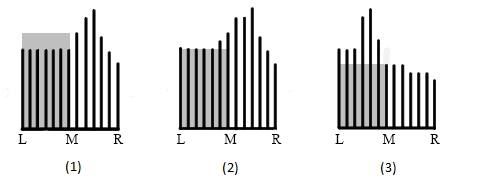
\includegraphics[width=9cm, height=3cm]{Term_3/Source/Pictures/Left.png}\\
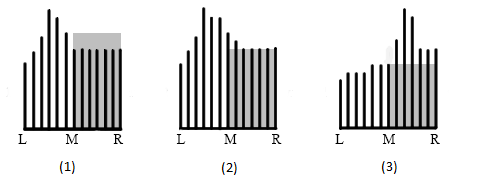
\includegraphics[width=9cm, height=3cm]{Term_3/Source/Pictures/Right2.png}\\
\end{frame}

\appendix
\section<presentation>*{\appendixname}
\subsection<presentation>*{Useful links}

\begin{frame}[allowframebreaks]
  \frametitle<presentation>{Полезные ссылки}
    
  \begin{thebibliography}{10}
{
  \beamertemplatebookbibitems
  % Start with overview books.
  
  \bibitem{kasai}
  \texttt{Викиконспекты: алгоритм Касаи}
  \newblock \href{https://bit.ly/2ygcpHb}{\texttt{https://bit.ly/2ygcpHb}}
  
    \bibitem{problem1}
  \texttt{Викиконспекты: алгоритм поиска подстроки в строке с помощью суффиксного массива}
  \newblock \href{https://bit.ly/2OahBqT}{\texttt{https://bit.ly/2OahBqT}}
  
      \bibitem{emaxx}
  \texttt{Emaxx: суффиксный массив}
  \newblock \href{http://e-maxx.ru/algo/suffix\_array}{\texttt{http://e-maxx.ru/algo/suffix\_array}}
  
}
    
  \end{thebibliography}
\end{frame}

\end{document}


